\documentclass{IFES-beamer}
\usepackage{url}
\usepackage{hyperref}

% --------------------------------------------------- %
%                  Presentation info	              %
% --------------------------------------------------- %
\title[Presentation Template]{Image retrieval using scene graphs}
\subtitle{Justin Johnson, Ranjay Krishna, Michael Stark, Li-Jia Li, David Shamma, Michael Bernstein, Li Fei-Fei}
\author{Ganga Meghanath \\ EE15B025}
\institute[IFES]{Stanford University, Max Planck Institute for Informatics, Yahoo Labs, Snapchat \\\\
  The IEEE Conference on Computer Vision and Pattern Recognition (CVPR), 2015, pp. 3668-3678\\
  (Cited by 212)
}
\date{\today}
\logo{

\includegraphics[scale=0.75]{logo.jpeg}
}
\subject{Presentation subject} % metadata

% --------------------------------------------------- %
%                    Title + Schedule                 %
% --------------------------------------------------- %

\begin{document}

\begin{frame}
  \titlepage
\end{frame}

\begin{frame}{Schedule}
  \tableofcontents
\end{frame}

% --------------------------------------------------- %
%                      Presentation                   %
% --------------------------------------------------- %

%%%%%%%%%%%%%%%%%%%%%%%%%%%%%%%%%%%%%%%%%%%%%%%%%%%%%%%%%%%%%%%%%%%%%%
\section{Problem Description}
    %----------------------------------------------------------
        \begin{frame}{Problem Statement}
            \begin{itemize}
                \item Retrieving images by describing their contents (objects, structured relationships and attributes)
                \item Utilize the structured nature of the query; perfect recognition of detailed semantics
            \end{itemize}
            \vspace{4mm}
            \begin{itemize}
                \item \textbf{Main challenges} : 
                    \begin{itemize}
                        \item Interactions between objects in a scene can be highly complex
                        \item Assumption of a closed universe (all classes are known beforehand) : does not hold
                    \end{itemize}
            \end{itemize}
            
        \end{frame}
        %----------------------------------------------------------
        \begin{frame}{Aim : Semantic image retrieval using a scene graph }
            \begin{itemize}
                \item \textbf{Scene Graph} explicitly models
                    \begin{itemize}
                        \item objects 
                        \item attributes of objects
                        \item relationships b/w objects 
                    \end{itemize}
            \end{itemize}
            \vspace{4mm}
            \begin{itemize}
                \item \textbf{Idea} : Perform semantic image retrieval using scene graphs as queries
                    \begin{itemize}
                        \item Scene graph used to represent the detailed semantics of a scene
                        \item Design Conditional Random Field  model (CRF model of visual scenes) grounding scene graphs to images 
                        \item The likelihoods - used as ranking scores for retrieval
                    \end{itemize}
            \end{itemize}
        \end{frame}
                    % \begin{table}[H]
                    %   \begin{center}
                    %     \begin{tabular}{|c|c|c|} % <-- Alignments: 1st column left, 2nd middle and 3rd right, with vertical lines in between
                    %     \hline
                    %     & Hawk & Dove\\
                    %       \hline
                    %       Hawk & $\frac{B-C}{2}, \frac{B-C}{2}$ & $B, 0$ \\
                    %       \hline
                    %       Dove & $0, B$ & $\frac{B}{2}, \frac{B}{2}$ \\
                    %       \hline
                    %     \end{tabular}
                    %   \end{center}
                    % \end{table}
%%%%%%%%%%%%%%%%%%%%%%%%%%%%%%%%%%%%%%%%%%%%%%%%%%%%%%%%%%%%%%%%%%%%%%
\section{Requirements}
    %$$$$$$$$$$$$$$$$$$$$$$$$$$$$$$$$$$$$$$$$$$$$$$$$$$$$$$$$$$$$$$
    \subsection{I/O}
        %----------------------------------------------------------
        \begin{frame}{Input - Output}
                \begin{itemize}
                    \item \textbf{Input Query} :  Scene Graph \vspace{5mm}
                    \item \textbf{Output} : Ranked retrieved images (in decreasing order of relevance)
                \end{itemize}
        \end{frame}
    
    %$$$$$$$$$$$$$$$$$$$$$$$$$$$$$$$$$$$$$$$$$$$$$$$$$$$$$$$$$$$$$$
    \subsection{Dataset}
        %----------------------------------------------------------
        \begin{frame}{Real-World Scene Graphs Dataset}
            \begin{itemize}
                \item Introduced a novel dataset of 5,000 human-generated scene graphs grounded to images; used to evaluate the method for image retrieval.
                \item The dataset consists of :
                    \begin{itemize}
                        \item 5,000 images
                        \item Over 93,000 object instances
                        \item  110,000 instances of attributes
                        \item 112,000 instances of relationships
                    \end{itemize}
                \item Per image statistics :
                    \begin{itemize}
                        \item Mean of 13.8 objects
                        \item Mean of 18.9 attributes
                        \item Mean of 21.9 relationships
                    \end{itemize}
            \end{itemize}
        \end{frame}
        
        %----------------------------------------------------------
        \begin{frame}{Real-World Scene Graphs Dataset}
            \begin{figure}
                \centering
                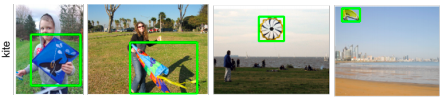
\includegraphics[width=9cm,height=8cm,keepaspectratio]{Images/scene_1.png}\\
                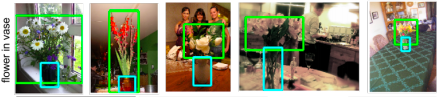
\includegraphics[width=9cm,height=8cm,keepaspectratio]{Images/scene_2.png}\\
                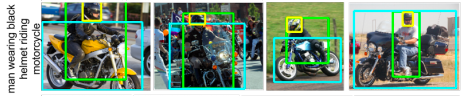
\includegraphics[width=9.5cm,height=8cm,keepaspectratio]{Images/scene_3.png}
                \caption{\cite{Johnson_2015_CVPR}Examples of scene sub-graphs of increasing complexity (top to bottom) from the Real-World Scene Graphs dataset, with attributes $\&$ different objects.}
                \label{fig:my_label}
            \end{figure}
        \end{frame}

%%%%%%%%%%%%%%%%%%%%%%%%%%%%%%%%%%%%%%%%%%%%%%%%%%%%%%%%%%%%%%%%%%%%%%
\section{Analytics}

    %----------------------------------------------------------
    \begin{frame}{Scene Graph and Grounding}
        \begin{itemize}
            \item \textbf{Scene Graph} :
                \begin{itemize}
                    \item A data structure that describes the contents of a scene
                    \item Given a set of object classes $C$, a set of attribute types $A$, and a set of relationship types $R$, a scene graph $\implies$ a tuple $G = (O, E)$ 
                        \begin{itemize}
                            \item $O = \{o_1, . . . , o_n\}$ is a set of objects
                            \item $E \subseteq O\times R\times O$ is a set of edges
                            \item  Each object, $o_i = (c_i, A_i)$ 
                            \item $c_i \in C$ is the class of the object
                            \item $A_i \sunseteq A$ are the attributes of the object
                        \end{itemize}  
                \end{itemize}
        \end{itemize}
        \begin{itemize}
            \item \textbf{Grounding a scene graph in an image}
                \begin{itemize}
                    \item A scene graph can be grounded to an image by associating each object instance of the scene graph to a region in an image.
                    \item Given a scene graph and an image, there are many possible ways of grounding the scene graph to the image.
                    \item A grounding of a scene graph $G = (O, E)$ is a map $\gamma : O \rightarrow B$ where an image is represented by a set of candidate bounding boxes $B$.
                \end{itemize}
        \end{itemize}
    \end{frame}
    
    %----------------------------------------------------------
    \begin{frame}{Depiction : Scene Graph and Grounding}
        \begin{figure}
            \centering
            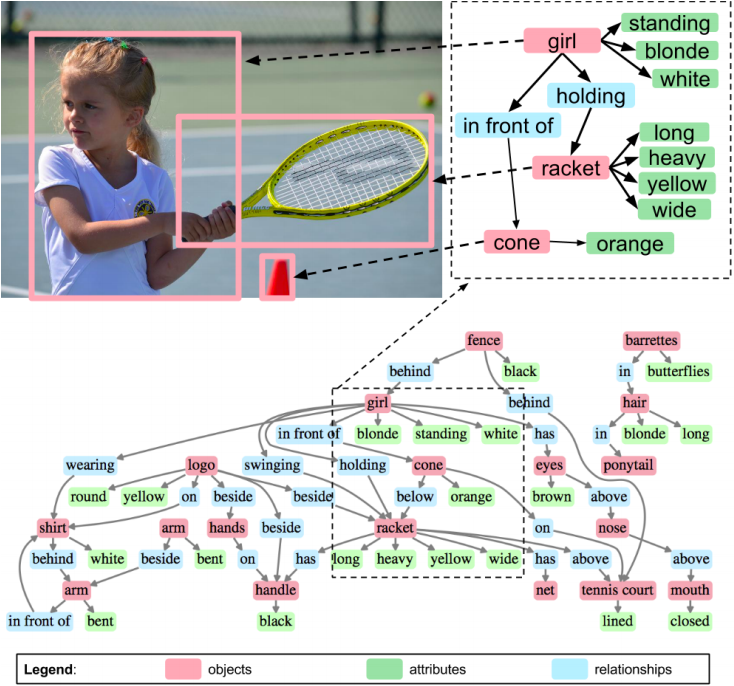
\includegraphics[scale=0.22]{Images/scene_graph.png}
            \caption{\cite{Johnson_2015_CVPR}An example of a scene graph (bottom) and a grounding (top). The scene graph encodes objects (“girl”), attributes, (“girl is blonde”), and relationships (“girl holding racket”). The grounding associates each object of the scene graph to a region of an image.}
            \label{fig:my_label}
        \end{figure}
    \end{frame}

    %----------------------------------------------------------
    \begin{frame}{Image Retrieval by Scene Graph Grounding}
        \begin{itemize}
            \item Use a scene graph as a query to retrieve images portraying scenes similar to the one described by the graph
            \item Measure the agreement between a query scene graph and an unannotated test image
            \item Conditional Random Field (CRF) models the distribution over all possible groundings
            \item MAP (Maximum a posteriori) estimate used to find the most likely grounding (measure of agreement between the scene graph and the image)
        \end{itemize}
    \end{frame}
    
    %----------------------------------------------------------
    \begin{frame}{Image Retrieval by Scene Graph Grounding}
        \begin{itemize}
            \item Use GOP(Geodesic Object Proposals)\cite{krahenbuhl2014geodesic} for generating candidate boxes for images (provides the best trade-off between object recall and number of regions per image).
            \item \textbf{CRF formulation} : \\
            Distribution over possible groundings, $$P(\gamma|G,B) = \prod_{o \in O} P(\gamma_o|o) \prod_{(o,r,o') \in E} P(\gamma_o, \gamma_{o'}|o,r,o')$$ 
            $$\gamma^{\star} = \underset{\gamma}{argmax} \prod_{o \in O} P(o|\gamma_o) \prod_{(o,r,o') \in E} P(\gamma_o, \gamma_{o'}|o,r,o')$$
            where $P(\gamma_o|o) = P(o|\gamma_o) \frac{P(\gamma_o)}{P(o)}$ by Bayes rule \\
            (Uniform prior $\implies P(\gamma_o), P(o)$ are constants)
        \end{itemize}
    \end{frame}
    
    %----------------------------------------------------------
    \begin{frame}{Image Retrieval by Scene Graph Grounding}
        \begin{itemize}
            \item \textbf{Unary potentials} : 
                \begin{itemize}
                    \item $P(o | \gamma_o)$ models how well the appearance of the box $\gamma_o$ agrees with the known object class and attributes of the object $o$. 
                    \item $$P(o|\gamma_o) = P(c|\gamma_o) \prod_{a \in A} P(a|\gamma_o)$$
                    \item R-CNN is used to train the detectors for each of the $|C| = 266$ and $|A| = 145$ object classes and attribute types. 
                    \item Platt scaling is used to convert the SVM classification scores for each object class and attribute into probabilities.
                \end{itemize}
        \end{itemize}
    \end{frame}
    
    %----------------------------------------------------------
    \begin{frame}{Image Retrieval by Scene Graph Grounding}
        \begin{itemize}
            \item \textbf{Binary potentials} : 
                \begin{itemize}
                    \item $P(\gamma_o, \gamma_{o'}|o,r,o')$ models how well the pair of bounding boxes $\gamma_o$, $\gamma_{o'}$ express the tuple $(o, r, o')$
                    \item $$f(\gamma_o, \gamma_{o'}) = \Big( (x-x')/w, (y-y')/h, w'/w, h'/h \Big)$$
                    where $\gamma_o = (x, y, w, h)$ and $\gamma_{o'} = (x', y', w', h')$ are the coordinates of the bounding boxes in the image
                    \item Train a Gaussian mixture model (GMM) to model $P(f(\gamma_o, \gamma_{o'})|c,r,c')$ where $c$ and $c'$ are classes of objects $o$ and $o'$.
                    \item Fewer than 30 instances of $(c,r,c')$ in the training data $implies$ use object agnostic model $P(f(\gamma_o, \gamma_{o'})|r)$
                    \item Use Platt scaling to convert the value of the GMM density function evaluated at $f(\gamma_o, \gamma_{o'})$ to a probability $P(\gamma_o, \gamma_{o'}|o,r,o')$
                \end{itemize}
        \end{itemize}
    \end{frame}
    
    %----------------------------------------------------------
    \begin{frame}{Methods used in Experiments}
        \begin{itemize}
            \item \textbf{SG-obj-attr-rel}: Model uses unary object and attribute potentials and binary relationship potentials.
            \item \textbf{SG-obj-attr}: Model uses only object and attribute potentials.
            \item \textbf{SG-obj}: Model uses only object potentials (object class potentials are rescaled R-CNN detection scores).
            \item \textbf{CNN}: L2 distance between the last layer features extracted using the reference model.
            \item \textbf{GIST}\cite{oliva2001modeling}: L2 distance between the GIST descriptors of the query image and each test image.
            \item \textbf{SIFT}\cite{lowe2004distinctive}
            \item \textbf{Random}: A random permutation of the test images.
        \end{itemize}
    \end{frame}
    
%%%%%%%%%%%%%%%%%%%%%%%%%%%%%%%%%%%%%%%%%%%%%%%%%%%%%%%%%%%%%%%%%%%%%%
\section{Results}
    %----------------------------------------------------------
    \begin{frame}{Results}
        \begin{figure}
            \centering
            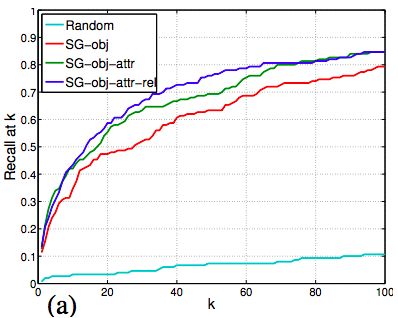
\includegraphics[scale=0.4]{Images/graph_a.png}
            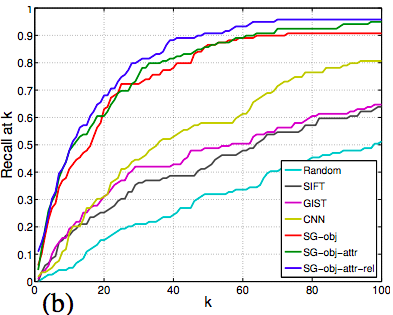
\includegraphics[scale=0.4]{Images/graph_b.png}
            \caption{\cite{Johnson_2015_CVPR}(a) Retrieval performance for entire scenes and (b) for partial scenes.}
            \label{fig:my_label}
        \end{figure}
    \end{frame}
    
    %----------------------------------------------------------
    \begin{frame}{Results}
        \begin{figure}
            \centering
            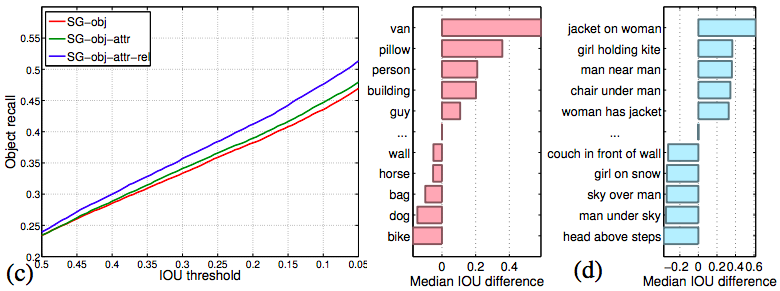
\includegraphics[scale=0.4]{Images/grapf_c_d.png}
            \caption{\cite{Johnson_2015_CVPR}(c) Object localization performance for entire scenes. (d) Increase in localization performance of our full model SG-obj-attr-rel vs SG-obj for individual objects (left) and objects participating in a relation (right). In (d), positive values indicate the SG-obj-attr-rel performs better than SG-obj}
            \label{fig:my_label}
        \end{figure}
    \end{frame}
    
     %----------------------------------------------------------
    \begin{frame}{Results}
        \begin{figure}
            \centering
            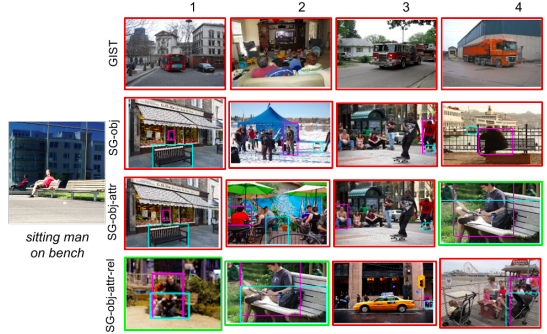
\includegraphics[scale=0.45]{Images/result3.png}
            \caption{\cite{Johnson_2015_CVPR}Top-4 retrieval results returned by different methods using a partial scene graph queries}
            \label{fig:my_label}
        \end{figure}
    \end{frame}
    
    %----------------------------------------------------------
    \begin{frame}{Results}
        \begin{itemize}
            \item Evaluation of image retrieval using full scene graphs and small scene subgraphs, shows that this outperforms retrieval methods that use only objects or low-level image features
            \item The full model can be used to improve object localization compared to baseline methods.
            \item Context provided by SG-obj-attr-rel helps to localize rare objects and objects with large appearance variations. 
            \item SG-obj-attr-rel gives large gains for tuples with well-defined spatial constraints.
        \end{itemize}
    \end{frame}
%%%%%%%%%%%%%%%%%%%%%%%%%%%%%%%%%%%%%%%%%%%%%%%%%%%%%%%%%%%%%%%%%%%%%%
\section{Criticism}
    %----------------------------------------------------------
        \begin{frame}{Novelty}
            \begin{itemize}
                \item Dataset : 5,000 human-annotated scene graphs grounded to images that use an open-world vocabulary to describe images in greater detail
            \end{itemize}
            \vspace{4mm}
            \begin{itemize}
                \item CRF model : semantic image retrieval using scene graph queries. Model outperforms baseline models that reason only about objects, and simple content-based image retrieval methods based on low-level visual features
            \end{itemize}
        \end{frame}
        
    %----------------------------------------------------------
    \begin{frame}{Pros}
        \begin{itemize}
            \item Replacing textual queries with scene graphs allows our queries to describe the semantics of the desired image in precise detail without relying on unstructured text.
            \item Using paragraph description for image retrieval (instead of scene graphs) would require the need to resolve co-references in the text, perform relationship extraction to convert the unstructured text into structured tuples, and ground the entities of the tuples into regions of the image described by the text.
            \item Can model multiple modes of interaction between pairs of objects while traditional CRF models are more restricted, and encode a fixed relation given two nodes.
            \item \textbf{Dataset} : contains significantly more labeled object instances per image than existing datasets, and also provides annotated attributes and relationships for individual object instances.
        \end{itemize}
    \end{frame}
    
    \begin{frame}{Cons}
        \begin{itemize}
            \item Requires the creation of a scene graph (Converting a description into a scene graph for query).
            \item Tuples encoding less well-defined spatial relationships may suffer in performance as the model penalizes valid configurations not seen at training time.
            \item Creation of training data is a cumbersome process (For each image : produce scene graph (using  Amazon’s Mechanical Turk - AMT), write (object, attribute) and (object, relationship, object) tuples using an open vocabulary to describe the image, draw bounding boxes for all objects, correct and verify the bounding boxes).
        \end{itemize}
    \end{frame}

%%%%%%%%%%%%%%%%%%%%%%%%%%%%%%%%%%%%%%%%%%%%%%%%%%%%%%%%%%%%%%%%%%%%%%
% \section{References}
    %----------------------------------------------------------
    % \nocite{Johnson_2015_CVPR}
    \begin{frame}{References}
        \printbibliography
    \end{frame}

    \begin{frame}{ }
        \begin{center}
            \Huge{\weva{\textbf{THANK YOU }}
            \textbf{:)}}
        \end{center}
        
    \end{frame}

\end{document}
